\documentclass[xcolor=dvipsnames,10pt]{beamer}
\usetheme{Madrid}
% \usefonttheme[onlymath]{serif}
\usepackage{pgfpages}
% \setbeameroption{show only notes}
\usepackage{amsmath, amsfonts, amssymb, amsthm}
\usepackage{bm, booktabs, graphicx, float}
\usepackage{mathtools}
\usepackage{tensor, hyperref, cleveref}
\usepackage[absolute,overlay]{textpos}
\usepackage{animate}
\usepackage{soul, multicol}
\usepackage{multimedia}
\makeatletter
\let\HL\hl
\renewcommand\hl{%
  \let\set@color\beamerorig@set@color
  \let\reset@color\beamerorig@reset@color
  \HL}
\makeatother
%SYMBOL DEFINITIONS
%
%
%===================================================================
% Boldface letters
%===================================================================
\def\bfa{{\bf a}}
\def\bfn{{\bf n}}
\def\bfm{{\bf m}}
\def\bfl{{\bf l}}
\def\bfu{{\bf u}}
\def\bfv{{\bf v}}
\def\bfx{{\bf x}}
\def\bfy{{\bf y}}
\def\bfz{{\bf z}}
\def\bfA{{\bf A}}
\def\bfE{{\bf E}}
\def\bfB{{\bf B}}
\def\bfC{{\bf C}}
\def\bfH{{\bf H}}
\def\bfI{{\bf I}}
\def\bfK{{\bf K}}
\def\bfL{{\bf L}}
\def\bfM{{\bf M}}
\def\bfN{{\bf N}}
\def\bfP{{\bf P}}
\def\bfQ{{\bf Q}}
\def\bfR{{\bf R}}
\def\bfS{{\bf S}}
\def\bfT{{\bf T}}
\def\bfX{{\bf X}}
\def\bfF{{\bf F}}
\def\bfU{{\bf U}}
\def\bfW{{\bf W}}
\def\bfY{{\bf Y}}
\def\bfZ{{\bf Z}}
%========================================================
% Greek bold face letters
%========================================================
\def\bfal{\mbox{\boldmath $\alpha$}}
\def\bfbe{\mbox{\boldmath $\beta$}}
\def\bfzeta{\mbox{\boldmath $\zeta$}}
\def\bfeps{\mbox{\boldmath $\epsilon$}}
\def\bfsig{\mbox{\boldmath $\sigma$}}
\def\bfD{{\bf D}}
\def\bfe{{\bf e}}
\def\bfg{\mbox{\boldmath $\gamma$}}
\def\bfG{\mbox{\boldmath $\Gamma$}}
\def\bfmu{\mbox{\boldmath $\mu$}}
\def\bfrho{{\bf S}}
\def\bfeta{\mbox{\boldmath $\eta$}}
\def\bfs{{\bf S}}
\def\bfXi{\mbox{\boldmath $\Xi$}}
\def\bfw{\mbox{\boldmath $\omega$}}
\def\bftau{\mbox{\boldmath $\tau$}}
\def\bfchi{\mbox{\boldmath $\chi$}}
\def\bfxi{\mbox{\boldmath $\xi$}}
\def\bfxip{\bfxi^{\perp}}
\def\bfG{\mbox{\boldmath $\Gamma$}}
\def\bfOm{\mbox{\boldmath $\Omega$}}
\def\Leff{\widetilde{\mbox{\boldmath$\mathcal{L}$}}}
\def\Ltan{\mbox{\boldmath$\mathcal{L}$}}
\def\Ktan{\mbox{\boldmath$\mathcal{K}$}}
\def\Jtan{\mbox{\boldmath$\mathcal{J}$}}
\def\Ctan{\mbox{\boldmath$\mathcal{C}$}}
\def\Mtan{\mbox{\boldmath$\mathcal{M}$}}
\def\Ptan{\mbox{\boldmath$\mathcal{P}$}}
\def\Qtan{\mbox{\boldmath$\mathcal{Q}$}}
\def\Stan{\mbox{\boldmath$\mathcal{S}$}}
\def\Atan{\mbox{\boldmath$\mathcal{A}$}}
\def\Itan{\mbox{\boldmath$\mathcal{I}$}}
\def\Htan{\mbox{\boldmath$\mathcal{H}$}}
\def\ehat{\hat{\bf e}}
%========================================================
% Greek letters
%========================================================
\def\a{\alpha}
\def\b{\beta}
\def\eps{\varepsilon}
\def\g{\gamma}
\def\l{\lambda}
\def\m{\mu}
\def\sig{\sigma}
\def\otheta{\overline{\theta}}
\def\oPsi{\overline{\Psi}}
\def\hPsi{\hat{\Psi}}
%========================================================
% Abbreviated forms
%========================================================
\def\eeq{\varepsilon_{e}}
\def\eem{\varepsilon_{m}}
\def\e0{\varepsilon_0}
\def\oQ{\overline{Q}}
\def\oR{\overline{R}}
\def\oS{\overline{S}}
\def\obfH{\overline{\bfH}}
\def\obfe{\overline{\bfeps}}
\def\obfeps{\overline{\bfeps}}
\def\bF{\overline{F}}
\def\oI{\overline{I}}
\def\oJ{\overline{J}}
\def\obfg{\overline{\bfg}}
\def\obfs{\overline{\bfs}}
\def\obfB{\overline{\bfB}}
\def\obfC{\overline{\bfC}}
\def\obfc{\overline{\bfc}}
\def\obfD{\overline{\bfD}}
\def\obfF{\overline{\bfF}}
\def\obfE{\overline{\bfE}}
\def\obfU{\overline{\bfU}}
\def\obfQ{\overline{\bfQ}}
\def\obfK{\overline{\bfK}}
\def\obfR{\overline{\bfR}}
\def\obfS{\overline{\bfS}}
\def\ol{\overline{\lambda}}
\def\oe{\overline{\varepsilon}}
\def\oos{\overline{\overline{\sigma}}}
\def\p{\partial}
\def\og{\overline{g}}
\def\oh{\overline{h}}
\def\oJ{\overline{J}}
\def\seq{\sigma_{eq}}
\def\sm{\sigma_{m}}
\def\s0{\sigma_0}
\def\v{\varphi}
\def\nn{\nonumber}
\def\Weff{\overline{W}}
\def\Pheff{\overline{\Phi}}
\def\meff{\overline{\mu}}
\def\keff{\overline{\kappa}}
\def\oL{\overline{\Lambda}}

\def\oH{\overline{H}}
\def\oF{\overline{F}}
\def\oL{\overline{L}}
\def\oLr{\overline{\Lr}}
\def\bfLr{{\bf \Lr}}
\def\bfwN{\bfw\otimes\bfxi}
\def\oJ{\overline{J}}

\def\obfS{\overline{\bfS}}
\def\obfF{\overline{\bfF}}
\def\obfH{\overline{\bfH}}
\def\obfL{\overline{\bfL}}
\def\obfLr{\overline{\bfLr}}
\def\cbfu{\check{\bfu}}
\def\cbfv{\check{\bfv}}

\def\Weff{\overline{W}}
\def\Ueff{\overline{U}}
%\def\Leff{\overline{\bfL}}
\def\Lreff{\overline{\Lr}}

\def\r{^{(r)}}
\def\p{\partial}

%Definitions: journals
\def\AMPA{{\it Ann. Mat. Pura Appl.\ }}
\def\AMR{{\it Appl. Mech. Rev.\ }}
\def\ARMA{Arch. Rat. Mech. Analysis\ }
\def\ASCEEM{{\it ASCE J. Eng. Mech.\ }}
\def\AAM{{\it Adv. Appl. Mech.\ }}
\def\CMAME {{\it Comput. Meth. Appl. Mech. Engrg.\ }}
\def\CS {{\it Comput. Struct.\ }}
\def\CRAS{C.R. Mecanique\ }
\def\EFM{{\it Eng. Fracture Mechanics\ }}
\def\EJMA{{\it Eur.~J.~Mechanics-A/Solids\ }}
\def\IJES{{\it Int. J. Eng. Sci.\ }}
\def\IJMS{{\it Int. J. Mech. Sci.\ }}
\def\IJNAMG{{\it Int. J. Numer. Anal. Meth. Geomech.\ }}
\def\IJP{{\it Int. J. Plasticity\ }}
\def\IJSS{Int. J. Solids Struct.\ }
\def\IngA{{\it Ing. Archiv\ }}
\def\JAM{{\it J. Appl. Mech.\ }}
\def\JAP{{\it J. Appl. Phys.\ }}
\def\JE{J. Elast.\ }
\def\JM{{\it J. de M\'ecanique\ }}
\def\JMPS{J. Mech. Phys. Solids\ }
\def\JPD{{\it J. Phys. D: Appl. Phys.\ }}
\def\MA{{\it Macromolecules\ }}
\def\MMS{{\it Math. Mech. Solids\ }}
\def\MOM{{\it Mech. Materials\ }}
\def\MRSSP{{\it Mat. Res. Soc. Symp. Proc.\ }}
\def\MTT{{\it Mekh. Tverd. Tela.\ }}
\def\MPCPS{{\it Math. Proc. Cambridge Phil. Soc.\ }}
\def\PRSLA{Proc. R. Soc. Lond. A\ }
\def\QAM{{\it Quart. Appl. Math.\ }}
\def\QJMAM{{\it Quart. J. Mech. Appl. Math.\ }}
\def\RAN{{\it Rend. Acc. Naz.\ }}
\def\RCT{{\it Rubb. Chem. Technol.\ }}

\def\doublelow#1{\,\vtop{\ialign{\hfil$##$\hfil\crcr
                    \mathstrut #1 \crcr}}\,}
\def\psiEq{\psi^{\rm Eq}}
\def\psiNEq{\psi^{\rm NEq}}
\newcommand{\croch}[1]{{\left[ #1 \right]}}
\newcommand{\accol}[1]{{\left\{ #1 \right\}}}
\newcommand{\del}[2]{\frac{\partial #1}{\partial #2}}
\newcommand{\ddel}[2]{\frac{\partial^2 #1}{\partial {#2}^2}}
\newcommand{\bigdel}[2]{\dfrac{\partial #1}{\partial #2}}
\newcommand{\lr}[1]{\left(#1\right)}
\long\def\symbolfootnote[#1]#2{\begingroup%
\def\thefootnote{\fnsymbol{footnote}}\footnote[#1]{#2}\endgroup}
\setlength{\parindent}{0pt}
% \usepackage{amsmath,amsfonts,amssymb}
% \usepackage[dvipsnames]{xcolor}
\newcommand\lrB[1]{{\left[#1 \right]}}
\hypersetup{
    colorlinks=true,
    linkcolor=red,
    citecolor=red,
    filecolor=magenta,      
    urlcolor=cyan,
    pdfpagemode=FullScreen,
}
% \setbeamerfont{title}{\normalfont}
% \makeatletter
% \def\insertsectionnavigation#1{%
%   \hbox to #1{\vbox{{\usebeamerfont{section in head/foot}%
%      \usebeamercolor[fg]{section in head/foot}%
%      \def\slideentry##1##2##3##4##5##6{}%
%      \def\sectionentry##1##2##3##4##5{%
%        \ifnum##5=\c@part%
%        \def\insertsectionhead{##2\hskip0.5em}%
%        \def\insertsectionheadnumber{##1}%
%        \def\insertpartheadnumber{##5}%
%          \hyperlink{Navigation##3}{%
%              \ifnum\c@section=##1%
%                {\usebeamertemplate{section in head/foot}}%
%              \else%
%                {\usebeamertemplate{section in head/foot shaded}}%
%              \fi%
%          }\par
%        \fi}%
%        \parbox[c][0cm][c]{.5\paperwidth}{%
%        \begin{multicols}{3}
%        \dohead
%        \end{multicols}}\space}
%      }%
%   \hfil}%
% }

% \def\insertsubsectionnavigation#1{%
%   \hbox to #1{%
%     \vbox{{%
%       \usebeamerfont{subsection in head/foot}\usebeamercolor[fg]{subsection in head/foot}%
%       \vskip0.5625ex%
%       \beamer@currentsubsection=0%
%       \def\sectionentry##1##2##3##4##5{}%
%       \def\slideentry##1##2##3##4##5##6{\ifnum##6=\c@part\ifnum##1=\c@section%
%         \ifnum##2>\beamer@currentsubsection%
%         \beamer@currentsubsection=##2%
%         \def\insertsubsectionhead{##5}%
%         \def\insertsectionheadnumber{##1}%
%         \def\insertsubsectionheadnumber{##2}%
%         \def\insertpartheadnumber{##6}%
%         \beamer@link(##4){%
%               \ifnum\c@subsection=##2%
%                 {\usebeamertemplate{subsection in head/foot}}%
%               \else%
%                 {\usebeamertemplate{subsection in head/foot shaded}}%
%               \fi\hfill}\par
%         \fi\fi\fi}%
%        \hspace*{0.5em}\parbox[c][0cm][c]{\dimexpr.5\paperwidth-1em\relax}{%
%        \begin{multicols}{4}
%        \dohead\vskip0.3625ex\end{multicols}
%        }\space
%    }\hfil
% }}}

% \setbeamertemplate{headline}
% {%
%   \leavevmode\@tempdimb=2.0075ex%
%   \ifnum\beamer@subsectionmax<\beamer@sectionmax%
%     \multiply\@tempdimb by\beamer@sectionmax%
%   \else%
%     \multiply\@tempdimb by\beamer@subsectionmax%
%   \fi%
%   \ifdim\@tempdimb>0pt%
%     \advance\@tempdimb by 1.005ex%
%     \begin{beamercolorbox}[wd=.5\paperwidth,ht=0.5\@tempdimb,dp=1.5ex]{section in head/foot}%
%       \vbox to0.5\@tempdimb{\vfill\insertsectionnavigation{.5\paperwidth}\vfill}%
%     \end{beamercolorbox}%
%     \begin{beamercolorbox}[wd=.5\paperwidth,ht=0.5\@tempdimb,dp=1.5ex]{subsection in head/foot}%
%       \vbox to0.5\@tempdimb{\vfill\insertsubsectionnavigation{.5\paperwidth}\vfill}%
%     \end{beamercolorbox}%
%   \fi%
% }
% \makeatother
\title[PINNs]{\large CS598: Physics-Informed Neural Networks:\\ A deep learning framework for solving forward and inverse problems involving nonlinear PDEs}
\author[M. Raissi, P. Perdikaris, GE. Karniadakis]{M. Raissi, P. Perdikaris, GE. Karniadakis \\[8pt] Bhavesh Shrimali}
\begin{document}
\begin{frame}
    \titlepage
\end{frame}
\AtBeginSection[]
{
  \begin{frame}[t]
    \frametitle{Table of Contents}
    \tableofcontents[currentsection]
  \end{frame}
}
\section{Introduction \& DNNs}
\begin{frame}[t]{Introduction: PINNs}
  \begin{itemize}
    \item<1-> PINNs - Neural networks that are trained to \hl{\bf solve supervised learning tasks while respecting physical laws (PDEs)}
    \begin{itemize}
      \item<2-> Data-driven solution \cite{raissi2017physicsI} 
      \item<3-> Data-driven discovery of PDEs \cite{raissi2017physicsII}
    \end{itemize}
    \item<4-> Two distinct types of algorithms
    \begin{itemize}
      \item<5-> New family of \emph{data-efficient} spatio-temporal function approximators 
      \item<6-> Arbitrary accurate RK time steppers with potentially unlimited number of stages
    \end{itemize}
    \item<7-> Paper: \cite{raissi2019physics}
  \end{itemize}
\end{frame}
\begin{frame}[t]{DNNs: Universal Approximators}
  \begin{itemize}
    \item<1-> Identify a nonlinear map from a few -- potentially very high dimensional -- input and output pairs of data
    \item<2-> However, many physical and biological systems consist of \hl{\bf prior knowledge encoded in physical laws}, e.g. Newton's laws of motion, Maxwell's laws of electromagnetism
    \item<3-> This prior information can act as \hl{\bf a regularization constraint} that reduces the space of admissible solutions $\implies$ \hl{\bf remove unrealistic solutions that violate fundamental conservation laws (mass, momentum, energy)}
    \item<4-> Previous ideas employed Gaussian process regression, but these were limited in their ability to handle nonlinear problems
  \end{itemize}

{\bf PDEs}
\begin{itemize}
  \item<5-> Need both initial conditions and boundary conditions
  \item<6-> Point Collocation methods: Function Approximation + point evaluation, e.g. consider an approximation problem for a function $u(x)$ on $x\in (0,1)$,
  $$
    u(x)\sim \widetilde{u}(x) = a_0 + a_1 x + a_2 x^2;\quad \text{with} \quad \widetilde{u}\lr{x_j} = \hat{u}_j,\, \, j=1,2
  $$
\end{itemize}
\end{frame}
\AtBeginSection[]
{
  \begin{frame}[t]
    \frametitle{Table of Contents}
    \tableofcontents[currentsection]
  \end{frame}
}
\section{Problem setup}
\begin{frame}[t]{Problem setup}
  \begin{itemize}
    \item<1-> Parameterized, nonlinear PDE(s)
    $$
      \color{BrickRed} u_{t}+\mathcal{N}[u ; \lambda]=0, x \in \Omega \subset \mathbb{R}^D,\, t \in[0, T];\quad \lr{\cdot}_t = \del{\lr{\cdot}}{t}
      \vspace*{-2ex}
    $$\vspace*{-2ex}
    \item<2-> where $u(t, x)$ denotes the latent (hidden) solution, $\mathcal{N}[\cdot ; \lambda]$ is a nonlinear operator parametrized by $\lambda$
    \item<3-> The above setup covers a wide range of PDEs in math. physics, including conservation laws, diffusion, reac-diff-advec. PDE, kinetics etc. E.g., {\color{blue} Burger's equation in 2D}
    $$
      \color{BrickRed}
      \mathcal{N}[u ; \lambda]=\lambda_{1} u u_{x}-\lambda_{2} u_{x x} \text { and } \lambda=\left(\lambda_{1}, \lambda_{2}\right);\quad \lr{\cdot}_{x} = \del{\lr{\cdot}}{x}
      \quad \lr{\cdot}_{xx} = \ddel{\lr{\cdot}}{x}
      \vspace*{-2ex}
    $$\vspace*{-2ex}
    \item<4-> Given $\lambda$ what is $u(t, x)$ (Inference, filtering and smoothing or simply \hl{\bf data-driven solutions of PDEs})
    \item<5-> Find $\lambda$ that best describes observations $u\lr{t_i, x_j}$ (Learning, system identification, or \hl{\bf data-driven discovery of PDEs})
  \end{itemize}
\end{frame}
\AtBeginSection[]
{
  \begin{frame}[t]
    \frametitle{Table of Contents}
    \tableofcontents[currentsection]
  \end{frame}
}
\section{Data driven solutions: Approach}
\begin{frame}[t]{Data-driven solutions}
  \begin{itemize}
    \item<1-> Rewrite the PDE as $f(u; t,x) = 0$
    $$
      f(u; t,x) \doteq u_{t}+\mathcal{N}[u], \quad \text{along with}\quad u = u_\theta \lr{t, x}
      \vspace*{-2ex}
      $$\vspace*{-2ex}
    \item<2-> Along with the above constraint (+ AD) this gives \emph{Physics-informed neural network} \hl{\bf parameterized by $\theta$}
    $$
      \mathcal{L}=\mathcal{L}_{u}+\mathcal{L}_{f}
    $$
    $$
      \mathcal{L}_{u}=\frac{1}{N_{u}} \sum_{i=1}^{N_{u}}\left|u\left(t_{u}^{i}, x_{u}^{i}\right)-u^{i}\right|^{2}\, ;\quad \mathcal{L}_{f}=\frac{1}{N_{f}} \sum_{i=1}^{N_{f}}\left|f\left(t_{f}^{i}, x_{f}^{i}\right)\right|^{2}
    $$
    \item<3-> $\left\{t_{u}^{i}, x_{u}^{i}, u^{i}\right\}_{i=1}^{N_{u}}$ denote the \hl{\bf initial and boundary training data} on $u(t, x)$
    \item<4-> $\left\{t_{f}^{i}, x_{f}^{i}\right\}_{i=1}^{N_{f}}$ specify the \hl{\bf collocation points}
    for $f(u;t,x)$
    \item<5-> $\mathcal{L}_u$ helps to enforce initial and boundary data accurately, while $\mathcal{L}_f$ imposes the structure of the PDE into the total loss
  \end{itemize}
\end{frame}
\AtBeginSection[]
{
  \begin{frame}[t]
    \frametitle{Table of Contents}
    \tableofcontents[currentsection]
  \end{frame}
}
\section{Data driven solutions: Example}
\begin{frame}[t]{Data-driven solutions: Examples}
  \begin{itemize}
    \item<1-> Most examples that follow have a small number of training data
    \begin{itemize}
      \item<2-> Optimizer: L-BFGS (quasi-second order)
      \item<3-> Full-batch
    \end{itemize}
    \item<4-> No theoretical guarantees, but as long as the PDE is well-posed $\implies$ optimizer will find the solution
  \end{itemize}
\end{frame}
\AtBeginSection[]
{
  \begin{frame}[t]
    \frametitle{Table of Contents}
    \tableofcontents[currentsection]
  \end{frame}
}
\section{Schr\"{o}dinger equation}
\begin{frame}[t]{Schr\"{o}dinger equation}
    \begin{itemize}
      \item<1-> Strong form of the PDE (note that \hl{$h(t, x) = u(t, x) + \mathrm{i}\, v(t,x)$})
      $$
      \begin{aligned}
        f\doteq \, &i h_{t}+0.5 h_{x x}+|h|^{2} h=0, \quad x \in[-5,5], \quad t \in[0, \pi / 2] \\
        &h(0, x)=2 \operatorname{sech}(x) \\
        &h(t,-5)=h(t, 5) \\
        &h_{x}(t,-5)=h_{x}(t, 5)
      \end{aligned}
    $$
    \item<2-> Total loss is given as
    $$
      \mathcal{L}
      =
      \underbrace{\mathcal{L}_{0}+\mathcal{L}_{b}}_{=\mathcal{L}_u}
      +
      \mathcal{L}_{f}
    $$
    \item<3-> Initial/Boundary data: 
    $$
      \begin{aligned}
        \mathcal{L}_{0}
      & =
      \frac{1}{N_{0}} \sum_{i=1}^{N_{0}}\left|h\left(0, x_{0}^{i}\right)-h_{0}^{i}\right|^{2}\, ;
      \qquad \mathcal{L}_{f}=\frac{1}{N_{f}} \sum_{i=1}^{N_{f}}\left|f\left(t_{f}^{i}, x_{f}^{i}\right)\right|^{2}
      \\
      \mathcal{L}_{b}
      & =
      \frac{1}{N_{b}} \sum_{i=1}^{N_{b}}\left(\left|h^{i}\left(t_{b}^{i},-5\right)-h^{i}\left(t_{b}^{i}, 5\right)\right|^{2}+\left|h_{x}^{i}\left(t_{b}^{i},-5\right)-h_{x}^{i}\left(t_{b}^{i}, 5\right)\right|^{2}\right)
      \end{aligned}
    $$
  \end{itemize}
\end{frame}
% \begin{frame}[t]{Schr\"{o}dinger equation}
%   \begin{block}{Schr\"{o}dinger equation}
%     \begin{itemize}
%       \item Strong form of the PDE
%       \vspace*{-1ex}
%       $$\vspace*{-2ex}
%       \begin{aligned}
%         f\doteq \, &i h_{t}+0.5 h_{x x}+|h|^{2} h=0, \quad x \in[-5,5], \quad t \in[0, \pi / 2] \\
%         &h(0, x)=2 \operatorname{sech}(x) \\
%         &h(t,-5)=h(t, 5) \\
%         &h_{x}(t,-5)=h_{x}(t, 5)
%       \end{aligned}
%     $$
%     \item Total loss is given as
%     \vspace*{-1ex}
%     $$\vspace*{-2ex}
%       \mathcal{L}
%       =
%       \underbrace{\mathcal{L}_{0}+\mathcal{L}_{b}}_{=\mathcal{L}_u}
%       +
%       \mathcal{L}_{f}
%     $$
%     \item<2-> Initial/Boundary data: 
%     $$\vspace*{-2ex}
%       \begin{aligned}
%         \mathcal{L}_{0}
%       & =
%       \frac{1}{N_{0}} \sum_{i=1}^{N_{0}}\left|h\left(0, x_{0}^{i}\right)-h_{0}^{i}\right|^{2}\\
%       \mathcal{L}_{b}
%       & =
%       \frac{1}{N_{b}} \sum_{i=1}^{N_{b}}\left(\left|h^{i}\left(t_{b}^{i},-5\right)-h^{i}\left(t_{b}^{i}, 5\right)\right|^{2}+\left|h_{x}^{i}\left(t_{b}^{i},-5\right)-h_{x}^{i}\left(t_{b}^{i}, 5\right)\right|^{2}\right)
%       \end{aligned}
%     $$
%   \end{itemize}
%   \end{block}
% \end{frame}
\begin{frame}[t]{Schr\"{o}dinger equation}
 
 {\bf Training data}
 \begin{itemize}
   \item<2-> Integrate the PDE using a Spectral solver \href{https://www.chebfun.org/}{(\texttt{Chebfun})} in space ($x$)
   \item<3-> A fourth order explicit RK time-stepper to integrate in time ($t$) \href{https://docs.scipy.org/doc/scipy/reference/generated/scipy.integrate.solve_ivp.html}{(\texttt{scipy.integrate.solve\_ivp})}
   \item<4-> $\left\{x_{0}^{i}, h_{0}^{i}\right\}_{i=1}^{N_{0}}$ are measurements of $h(t, x)$ at time $t=0$. Specifically they choose, $N_0 = N_b = 50$ and $N_f = 20,000$
 \end{itemize}

 \vspace*{1ex}
 {\bf Representation}
 \begin{itemize}
   \item<5-> $h(t, x)=[u(t, x) v(t, x)]$ using a $5$-layer deep neural network with $100$ neurons per layer
   \item<6-> The choice is purely empricial (no theoretical basis (yet)). Bayesian optimization to fine-tune the design of the DNN
 \end{itemize}

 \vspace*{1ex}
 {\bf Potential issues}
 \begin{itemize}
   \item<7-> Continuous time NN models require a large number of collocation points through the domain $N_f$
 \end{itemize}

\end{frame}
\begin{frame}[t]{Schr\"{o}dinger equation}
  \begin{figure}
    \centering
    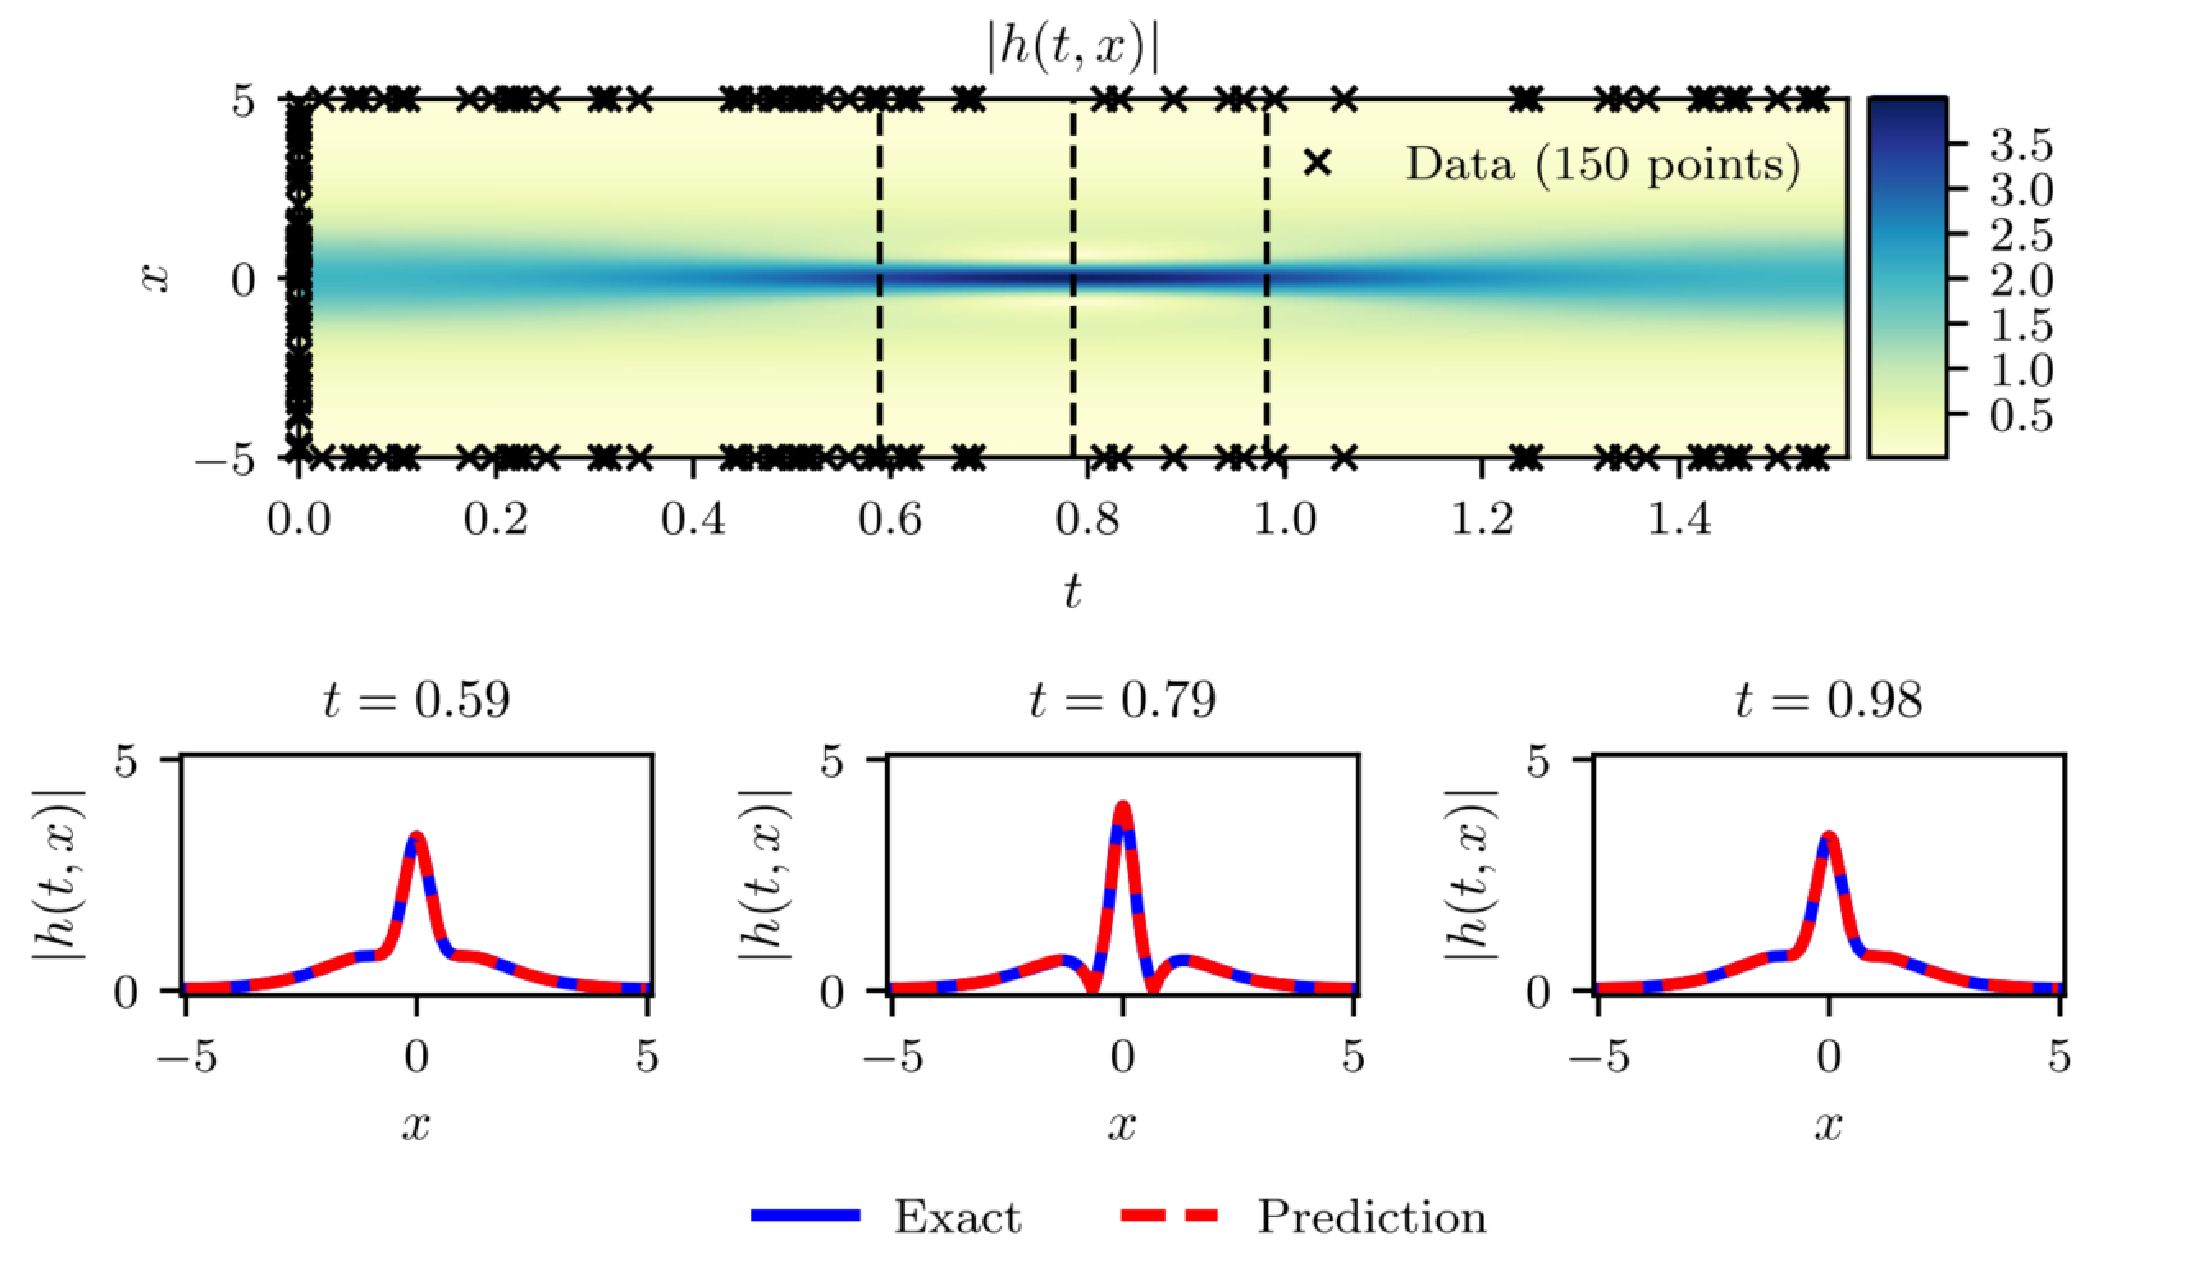
\includegraphics[width=0.9\linewidth]{h_tx.eps}
    \caption{
      \centering
      Top: Boundary and Initial data ($150$ points), Bottom: Snapshots of the solution of the Schr\"{o}dinger equation using a PINN
    }
  \end{figure}
\end{frame}
\begin{frame}[t]{Schr\"{o}dinger equation}
  
  {\bf Flexible time-steppers:}
  \begin{itemize}
    \item<2-> Use a generalized RK method with, say, $q$ stages
    $$
      \begin{aligned}
      &u^{n+c_{i}}=u^{n}-\Delta t \sum_{j=1}^{q} a_{i j} \mathcal{N}\left[u^{n+c_{j}}\right], \quad i=1, \ldots, q \\
      &u^{n+1}=u^{n}-\Delta t \sum_{j=1}^{q} b_{j} \mathcal{N}\left[u^{n+c_{j}}\right]
      \end{aligned}
    $$
      \item<3-> The above update can be rewritten as
      $$
        u^{n}=u_{i}^{n}, \quad i=1, \ldots, q\, ;  \quad \text{and}\quad u^{n}=u_{q+1}^{n}
      $$
      with
      $$
        \begin{aligned}
          &u_{i}^{n}\doteq 
          u^{n+c_{i}}+\Delta t \sum_{j=1}^{q} a_{i j} \mathcal{N}\left[u^{n+c_{j}}\right], \quad i=1, \ldots, q \\
          &u_{q+1}^{n}\doteq 
          u^{n+1}+\Delta t \sum_{j=1}^{q} b_{j} \mathcal{N}\left[u^{n+c_{j}}\right]
        \end{aligned}
      $$ 
  \end{itemize}
\end{frame}
\AtBeginSection[]
{
  \begin{frame}[t]
    \frametitle{Table of Contents}
    \tableofcontents[currentsection]
  \end{frame}
}
\section{Allen-Cahn equation}
\begin{frame}[t]{Allen-Cahn Equation}
  \begin{itemize}
    \item<2-> Make use of the above adaptive time-stepper
    $$
      \begin{aligned}
        &u_{t}-0.0001 u_{x x}+5 u^{3}-5 u=0, \quad x \in[-1,1], \quad t \in[0,1], \\
        &u(0, x)=x^{2} \cos (\pi x), \\
        &u(t,-1)=u(t, 1), \\
        &u_{x}(t,-1)=u_{x}(t, 1) .
      \end{aligned}
    $$
    \item<3-> The differential operator: $\mathcal{N}\left[u^{n+c_{j}}\right]=-0.0001 u_{x x}^{n+c_{j}}+5\left(u^{n+c_{j}}\right)^{3}-5 u^{n+c_{j}}$
    \item<4-> The loss function is the sum of squared losses 
    $$
      S S E_{n}=\sum_{j=1}^{q+1} \sum_{i=1}^{N_{n}}\left|u_{j}^{n}\left(x^{n, i}\right)-u^{n, i}\right|^{2}
    $$
    $$
      \begin{aligned}
        S S E_{b}
        &=
        \sum_{i=1}^{q}\left|u^{n+c_{i}}(-1)-u^{n+c_{i}}(1)\right|^{2}+\left|u^{n+1}(-1)-u^{n+1}(1)\right|^{2} \\
        &+
        \sum_{i=1}^{q}\left|u_{x}^{n+c_{i}}(-1)-u_{x}^{n+c_{i}}(1)\right|^{2}+\left|u_{x}^{n+1}(-1)-u_{x}^{n+1}(1)\right|^{2}
      \end{aligned}
    $$
  \end{itemize}
\end{frame}
\begin{frame}[t]{Allen-Cahn Equation}
  \begin{figure}[H]
    \centering
    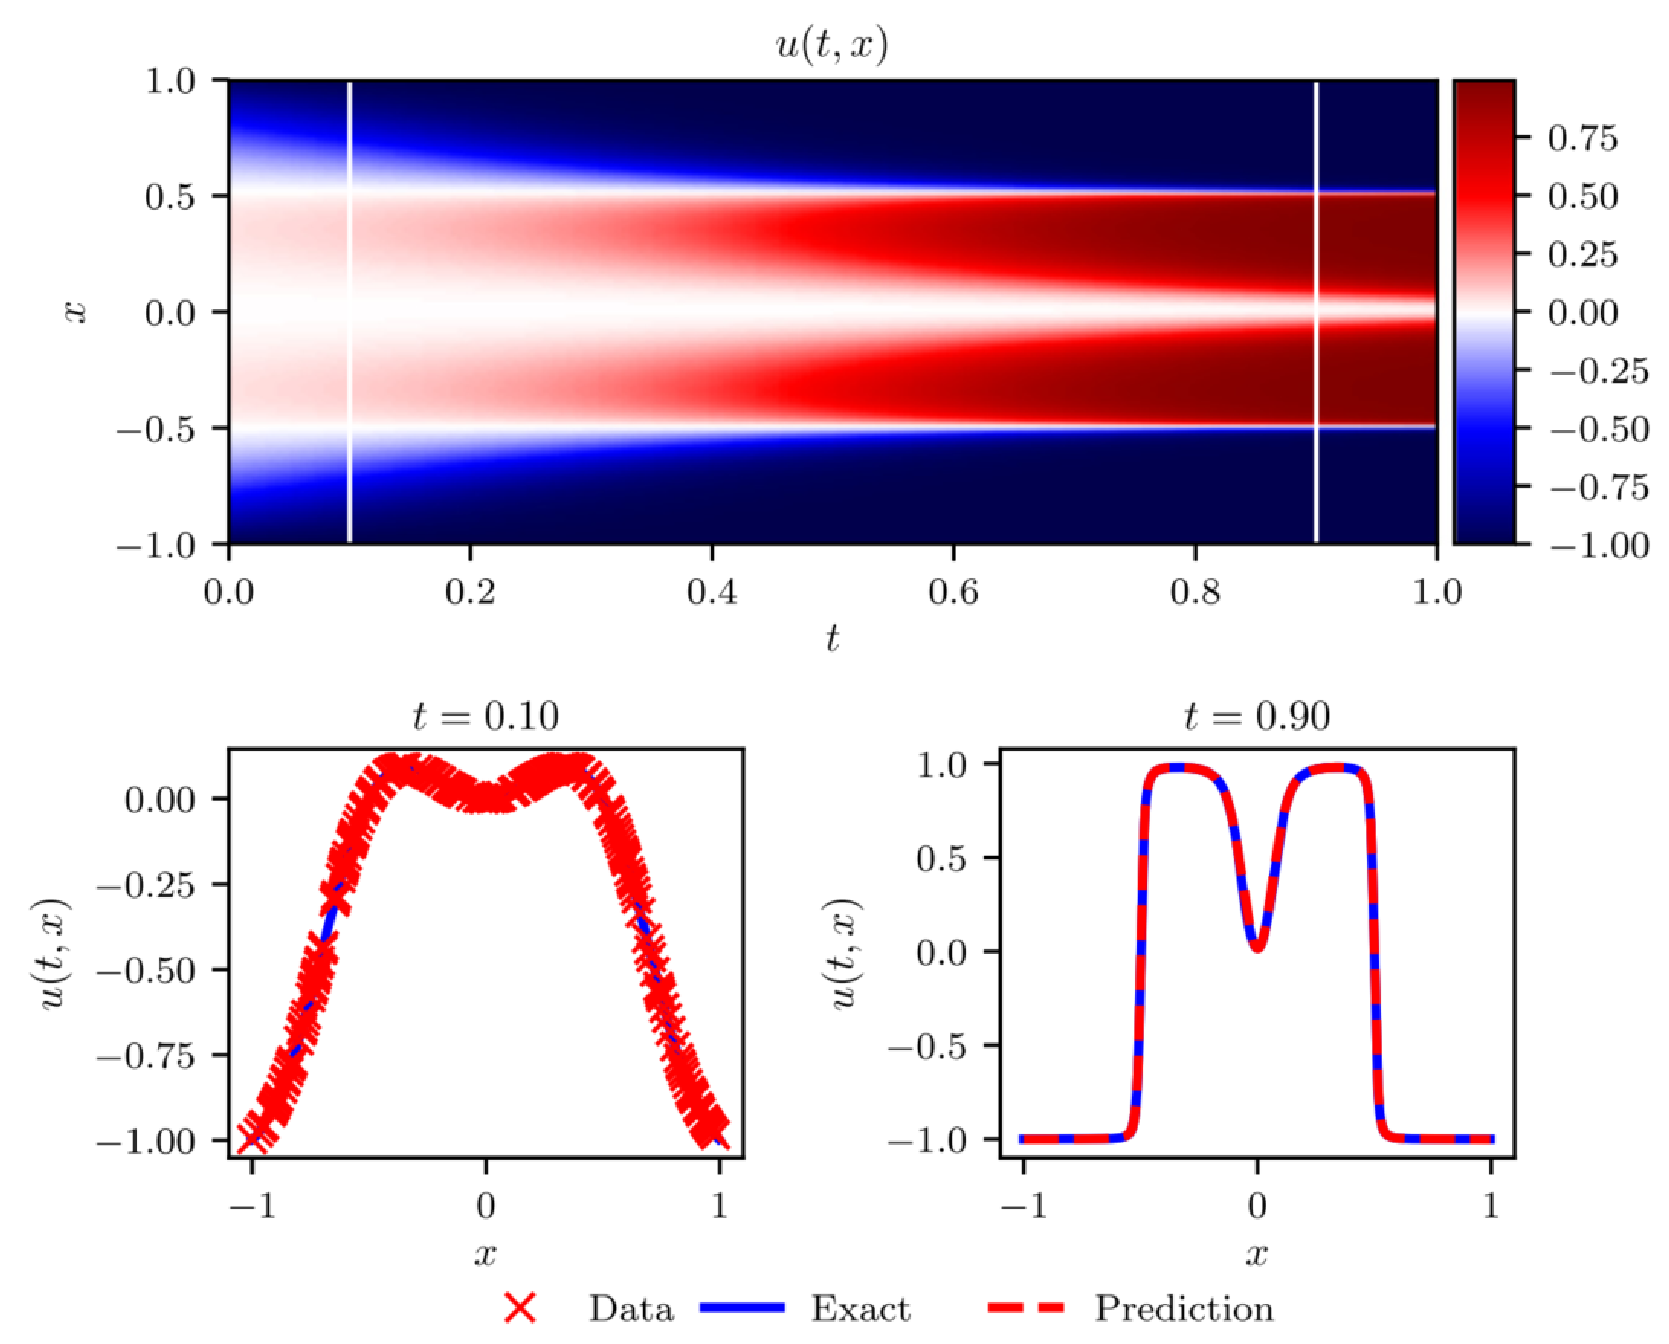
\includegraphics[width=0.7\linewidth]{u_tx.eps}
  \end{figure}
\end{frame}
\AtBeginSection[]
{
  \begin{frame}[t]
    \frametitle{Table of Contents}
    \tableofcontents[currentsection]
  \end{frame}
}
\section{Data-driven discovery: Navier Stokes}
\begin{frame}[t]{Data-driven discovery of PDEs: Navier Stokes}
  
  {\bf Navier-Stokes Equations}
  \begin{itemize}
    \item<2-> Describe the physics of many phenomena, such as weather, ocean currents, water flow in a pipe and air flow around a wing.
    $$
      \begin{aligned}
      &u_{t}+\lambda_{1}\left(u u_{x}+v u_{y}\right)=-p_{x}+\lambda_{2}\left(u_{x x}+u_{y y}\right) \\
      &v_{t}+\lambda_{1}\left(u v_{x}+v v_{y}\right)=-p_{y}+\lambda_{2}\left(v_{x x}+v_{y y}\right)
      \end{aligned};\quad \text{where}\quad \lr{\cdot}_x = \frac{\partial\lr{\cdot}}{\partial x}
    $$
    \item<3-> $u(t, x, y)$ denotes the $x$-component of the velocity, $v(t, x, y)$ denotes the $y$ component and $p(t, x, y)$ the pressure
    \item<4-> Conservation of mass: $u_{x}+v_{y}=0 \implies$ $u=\psi_{y}, \quad v=-\psi_{x}$
    \item<5-> Given a set of observations: $\left\{t^{i}, x^{i}, y^{i}, u^{i}, v^{i}\right\}_{i=1}^{N}$
    $$
      \begin{aligned}
      &f \doteq u_{t}+\lambda_{1}\left(u u_{x}+v u_{y}\right)+p_{x}-\lambda_{2}\left(u_{x x}+u_{y y}\right) \\
      &g \doteq v_{t}+\lambda_{1}\left(u v_{x}+v v_{y}\right)+p_{y}-\lambda_{2}\left(v_{x x}+v_{y y}\right)
      \end{aligned}
    $$
    \item<6-> Learn $\lambda = \{\lambda_1, \lambda_2\}$, and pressure field $p(t, x, y)$ by jointly approximating $[\psi(t, x, y) \quad p(t, x, y)]$ with a single NN with two outputs 
  \end{itemize}
\end{frame}
\begin{frame}[t]{Data-driven discovery of PDEs: Navier Stokes}
  
  {\bf Navier-Stokes Equations}
  \begin{itemize}
    \item<2-> Train by minimizing the total loss 
    $$
    \begin{aligned}  
      \mathcal{L}
      &\doteq
        \frac{1}{N} \sum_{i=1}^{N}\left(\left|u\left(t^{i}, x^{i}, y^{i}\right)-u^{i}\right|^{2}+\left|v\left(t^{i}, x^{i}, y^{i}\right)-v^{i}\right|^{2}\right) \\
      &+
        \frac{1}{N} \sum_{i=1}^{N}\left(\left|f\left(t^{i}, x^{i}, y^{i}\right)\right|^{2}+\left|g\left(t^{i}, x^{i}, y^{i}\right)\right|^{2}\right)
      \end{aligned}
    $$
    \item<3-> Consider the prototypical problem of an incompressible flow past a (rigid) cylinder, with various values of the Reynolds number $R e=u_{\infty} D / \nu$
    \item<4-> Training data is generated using a high-res spectral solver \href{https://www.nektar.info/}{(\texttt{NekTar})}
    \item<5-> Higher order piecewise approximation in space (tenth-order jacobi polynomials), third-order approximation in time (stable for stiff problems)
    \item<6-> Given stream-wise $u(t, x, y)$ and transverse $v(t, x, y)$ velocity data, identify unknown $\lambda = \{\lambda_1, \lambda_2\}$ as well as reconstruct $p(t, x, y)$
  \end{itemize}
\end{frame}
\begin{frame}[t]{Navier-Stokes PDE}
  \begin{figure}[H]
    \centering
    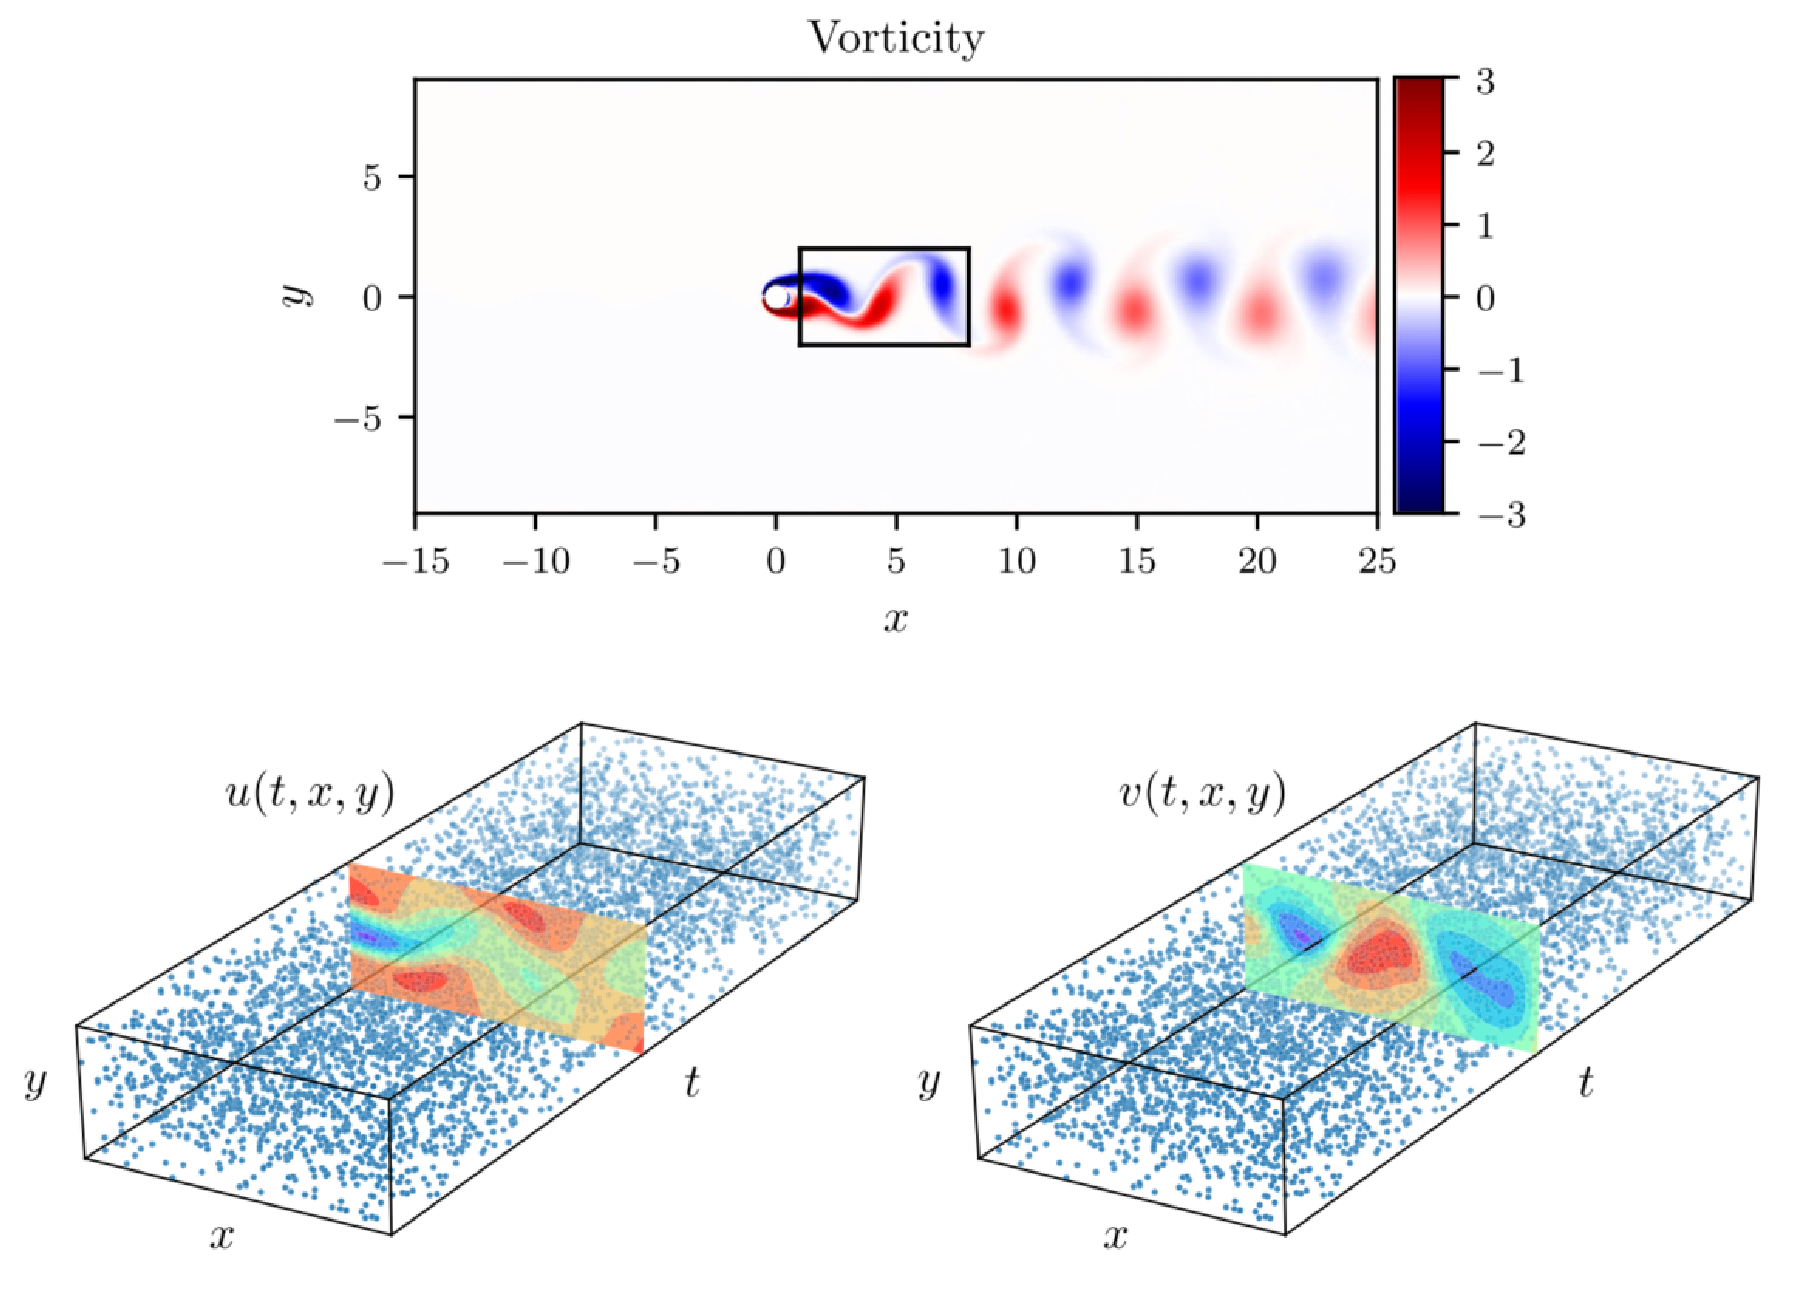
\includegraphics[width=0.65\linewidth]{vorticity.eps}
    \caption{\footnotesize\centering
      Navier-Stokes equation: \textbf{Top}: Incompressible flow and dynamic vortex shedding past a circular cylinder at Re $=100$. The spatio-temporal training data correspond to the depicted rectangular region in the cylinder wake. \textbf{Bottom}: \hl{Locations of training data-points for the stream-wise and transverse velocity components}, $u(t, x, y)$ and $v(t, x, t)$, respectively.
    }
  \end{figure}
\end{frame}
\begin{frame}[t]{Navier-Stokes PDE: Observations}
  \begin{itemize}
    \item<1-> Set $N = 5000\sim$1\% of the total available data
    \begin{figure}[H]
      \centering
      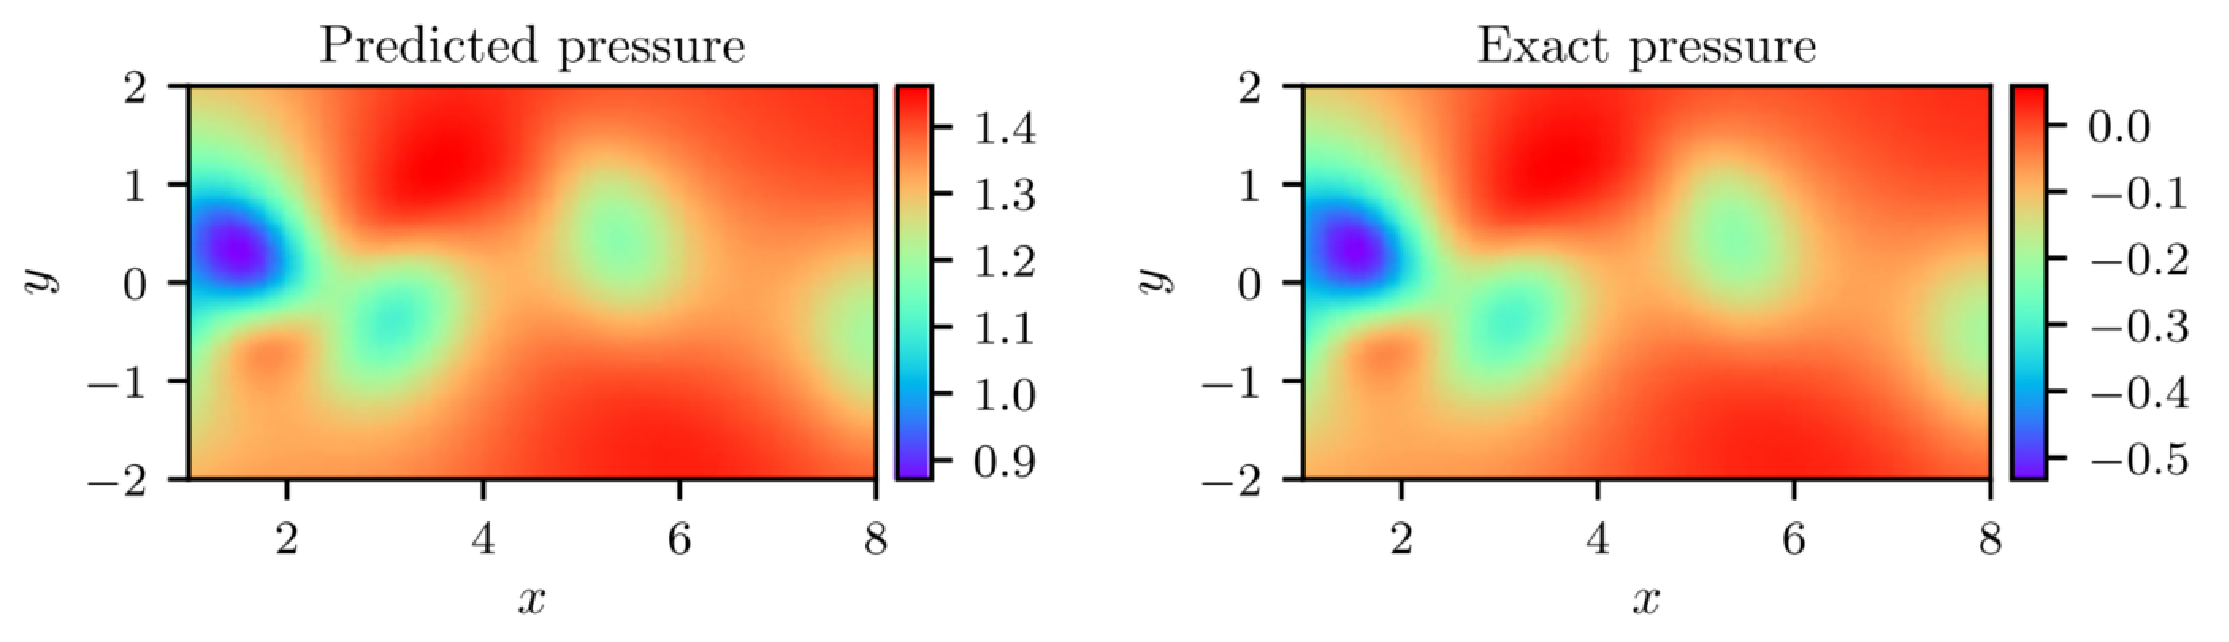
\includegraphics[width=0.9\linewidth]{pressurePredicted.eps}
      \caption{\footnotesize\centering
        Results for predicted pressure field}
    \end{figure}
    \begin{table}
      \centering\footnotesize
      \begin{tabular}{|c|c|}
        \hline Correct PDE & $u_{t}+\left(u u_{x}+v u_{y}\right)=-p_{x}+0.01\left(u_{x x}+u_{y y}\right)$ \\
        & $v_{t}+\left(u v_{x}+v v_{y}\right)=-p_{y}+0.01\left(v_{x x}+v_{y y}\right)$ \\
        \hline Identified PDE (clean data) & $u_{t}+0.999\left(u u_{x}+v u_{y}\right)=-p_{x}+0.01047\left(u_{x x}+u_{y y}\right)$ \\
        & $v_{t}+0.999\left(u v_{x}+v v_{y}\right)=-p_{y}+0.01047\left(v_{x x}+v_{y y}\right)$ \\
        \hline Identified PDE (1\% noise) & $u_{t}+0.998\left(u u_{x}+v u_{y}\right)=-p_{x}+0.01057\left(u_{x x}+u_{y y}\right)$ \\
        & $v_{t}+0.998\left(u v_{x}+v v_{y}\right)=-p_{y}+0.01057\left(v_{x x}+v_{y y}\right)$ \\
        \hline
        \end{tabular}
        \caption{\centering
          Correct partial differential equation along with the identified one obtained by learning $\lambda_1, \lambda_2$ and $p(t, x, y)$.
        }
    \end{table}
  \end{itemize}
\end{frame}
\AtBeginSection[]
{
  \begin{frame}[t]
    \frametitle{Table of Contents}
    \tableofcontents[currentsection]
  \end{frame}
}
\section{Korteweg-de Vries equation}
\begin{frame}[t]{Korteweg-de Vries equation}
  \begin{itemize}
    \item<2-> \textrm{KdV} equation has higher order derivatives (models shallow water waves)
    $$
      u_{t}+\lambda_{1} u u_{x}+\lambda_{2} u_{x x x}=0
    $$
    \item<3-> Learn a set of parameters (similar to NS)
    $$
      \mathcal{N}\left[u^{n+c_{j}}\right]=\lambda_{1} u^{n+c_{j}} u_{x}^{n+c_{j}}-\lambda_{2} u_{x x x}^{n+c_{j}}
    $$
    \begin{figure}[H]
      \centering
      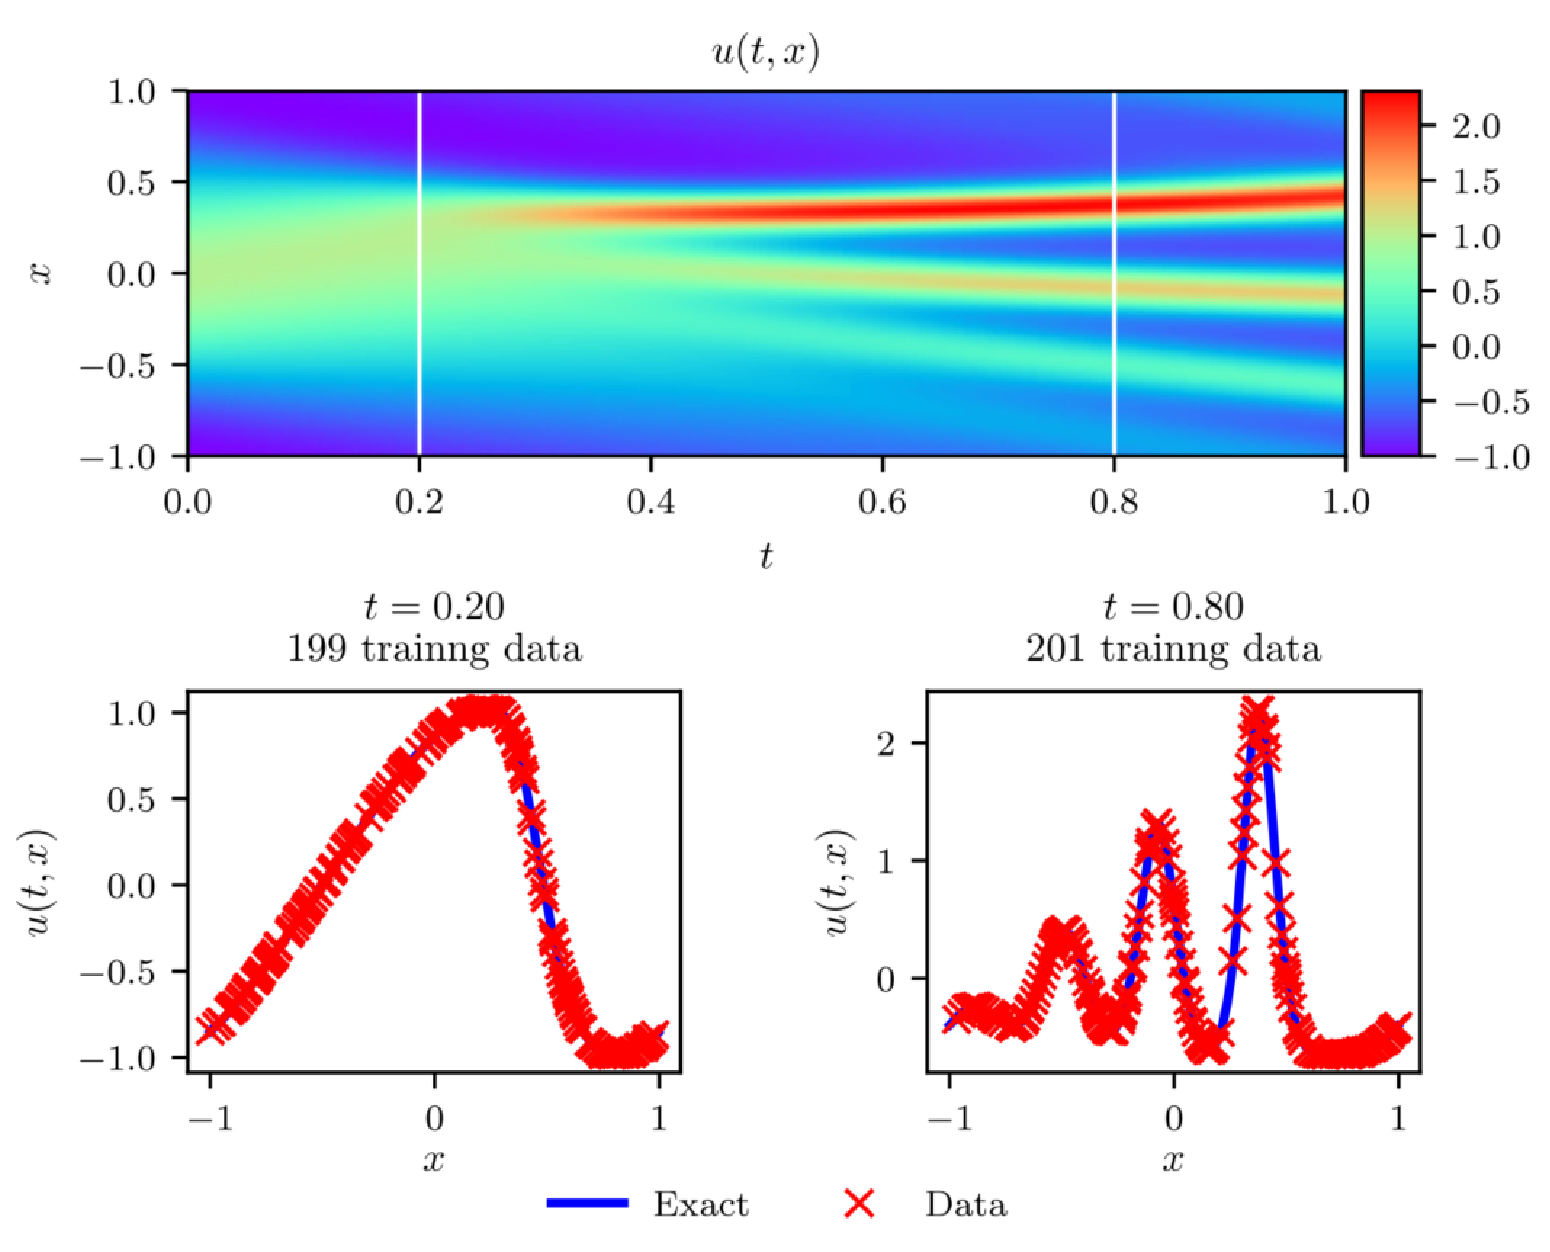
\includegraphics[width=0.6\linewidth]{utx2.eps}
      \caption{\footnotesize\centering
        Results for the KdV equation}
    \end{figure}
  \end{itemize}
\end{frame}
\begin{frame}[t]{Korteweg-de Vries equation}
  \begin{table}
    \centering
    \begin{tabular}{|c|c|}
      \hline Correct PDE & $u_{t}+u u_{x}+0.0025 u_{x x x}=0$ \\
      \hline Identified PDE (clean data) & $u_{t}+1.000 u u_{x}+0.0025002 u_{x x x}=0$ \\
      \hline Identified PDE (1\% noise) & $u_{t}+0.999 u u_{x}+0.0024996 u_{x x x}=0$ \\
      \hline
      \end{tabular}
  \end{table}

  {\bf Remarks}

  \begin{itemize}
    \item<2-> Traditional spectral solvers require a smaller time-increment to achieve similar accuracy
    \item<3-> The authors chose $q$ (hyperparameter) using a tolerance $\epsilon$ (in this case set to machine precision)
    $$
      q=0.5 \log \epsilon / \log (\Delta t)
    $$
    \item<4-> Time step for this problem is $\Delta t = 0.6$
    \item<5-> For the case of noise-free training data, the error in estimating $\lambda_{1}$ and $\lambda_{2}$ is $0.023 \%$, and $0.006 \%$, respectively, while the case with $1 \%$ noise in the training data returns errors of $0.057 \%$, and $0.017 \%$, respectively.
    \item<6-> Even for large temporal variations in the solution, the model is able to resolve the dynamics accurately
  \end{itemize}
\end{frame}
\AtBeginSection[]
{
  \begin{frame}[t]
    \frametitle{Table of Contents}
    \tableofcontents[currentsection]
  \end{frame}
}
\section{Conclusion}
\begin{frame}[t]{Conclusion}
  \begin{itemize}
    \item<2-> Introduced physics-informed neural networks, a new class of universal function approximators that are capable of encoding any underlying physical laws that govern a given data-set (described by PDEs)
    \item<3-> Design data-driven algorithms for inferring solutions to general nonlinear PDEs, and constructing computationally efficient physics-informed surrogate models.
  \end{itemize}

  {\bf Questions}
  \begin{itemize}
    \item<4-> How deep/wide should the neural network be ? How much data is really needed ?
    \item<5-> Why does the algorithm converge to unique values for the parameters of the differential operators, i.e., why is the algorithm not suffering from local optima for the parameters of the differential operator?
    \item<6-> Does the network suffer from vanishing gradients for deeper architectures and higher order differential operators? Could this be mitigated by using different activation functions?
    \item<7-> Can we improve on initializing the network weights or normalizing the data? Loss function choices (MSE, SSE)? Robustness? 
  \end{itemize}
\end{frame}
\begin{frame}[t]{Code}
  \begin{itemize}
    \item<2-> \url{https://github.com/maziarraissi/PINNs} (TensorFlow)
    \item<3-> Blog: \url{https://maziarraissi.github.io/PINNs/}
    \item<4-> \texttt{NeuralPDE.jl}: \url{https://neuralpde.sciml.ai/dev/}
    \item<5-> \texttt{IDRLNet}: \url{https://github.com/idrl-lab/idrlnet} (PyTorch)
  \end{itemize}
\end{frame}
\begin{frame}[t]{References}
  \footnotesize
    \bibliographystyle{icml2021}
    \bibliography{references}
\end{frame}
\end{document}